\documentclass[handout]{beamer}
%\documentclass{beamer}
\usepackage{tikz}
\def\checkmark{\tikz\fill[scale=0.4](0,.35) -- (.25,0) -- (1,.7) -- (.25,.15) -- cycle;} 
\usepackage{pifont}
\newcommand{\xmark}{\ding{55}}
\usepackage{tikz}
\usepackage{biblatex}
\usetheme{PaloAlto}
\title{A romp through MCMC}
\author[Ben Lambert]{Ben Lambert\inst{1}\\ \texttt{ben.c.lambert@gmail.com}}
\usepackage{datetime}
\date{}
\institute[University of Oxford]{
	\inst{1}University of Oxford}
\beamertemplatenavigationsymbolsempty
\setbeamertemplate{sidebar left}{}
\usepackage{caption}
\captionsetup{font=footnotesize}
\usepackage[utf8]{inputenc}
\usepackage{amsmath}
\usepackage{multimedia}
\usepackage{animate}
\usepackage{graphics}
\usepackage{graphicx}
\usepackage[makeroom]{cancel}

\makeatletter
\newcommand\mathcircled[1]{%
  \mathpalette\@mathcircled{#1}%
}
\newcommand\@mathcircled[2]{%
  \tikz[baseline=(math.base)] \node[draw,circle,inner sep=1pt] (math) {$\m@th#1#2$};%
}
\makeatother

\bibliography{Bayes}

\begin{document}

\begin{frame}
\titlepage
\end{frame}

\begin{frame}
\frametitle{Lecture outcomes}

\begin{enumerate}
\item<2-> Appreciate how sampling can be used to gain insight into a distribution.
\item<3-> Grasp how \textbf{dependent sampling} via \textbf{MCMC} allows sampling from the posterior.
\item<4-> Understand the mechanics of Random Walk Metropolis and how it works intuitively.
\item<5-> Know that judging convergence of chains to the posterior is \textit{hard}.
\item<6-> Learn how adaptive covariance MCMC and Hamiltonian Monte Carlo can speed up sampling in most cases.
\item See how to formulate the inference problem for ODEs and PDEs.
\item Understand how ABC works.
\end{enumerate}

\end{frame}

\section{Understanding a distribution by sampling from it}
\frame{\tableofcontents[currentsection]}

\begin{frame}
\frametitle{What is (independent) sampling and how can it give insight to distributions?}
\begin{itemize}
\item<2-> Suppose we have a large (infinite) urn filled with coloured balls.
\item<3-> The number of colours and the frequencies of each are \textbf{unknown}.
\item<4-> \textbf{Question:} how can we determine the underlying probability distribution of ball colour?
\end{itemize}

\onslide<1->
\begin{figure}[t]
\centerline{\animategraphics[autoplay,loop,width=0.8\textwidth,controls,buttonsize=1em,buttonfg=0.5]{2}{animations_figures/lec4_urn}{1}{10}}
\end{figure}

\end{frame}

\begin{frame}
\frametitle{What is (independent) sampling and how can it give insight to distributions?}
\onslide<1-> \textbf{Answer:} we draw lots of balls from the urn and count the \textbf{sampled} frequencies!

\onslide<2-> 

\begin{figure}[t]
\centerline{\animategraphics[width=1\textwidth,controls,buttonsize=1em,buttonfg=0.5]{8}{animations_figures/lec4_urnSampling}{1}{101}}
\end{figure}

\end{frame}

\begin{frame}
\frametitle{What is (independent) sampling and how can it give insight to distributions?}

\begin{itemize}
\item<2-> Drawing one ball from the urn is the act of taking a single \textbf{sample}.
\item<3-> If the balls in the urn are swishing about then the colour of the next ball does not depend on the current ball's colour.
\item<4-> Here the samples are (conditionally-) \textbf{independent}.
\item<5-> Independent sampling gives us a very \textbf{efficient} way of gaining insight into a distribution.
\end{itemize}

\onslide<1->
\begin{figure}[t]
\centerline{\animategraphics[autoplay,loop,width=0.8\textwidth,controls,buttonsize=1em,buttonfg=0.5]{2}{animations_figures/lec4_urn}{1}{10}}
\end{figure}

\end{frame}

\begin{frame}
\frametitle{Sampling from a continuous distribution}
\begin{itemize}
\item<2-> Suppose we have a large (infinite) urn filled with balls of differing sizes.
\item<3-> The distribution of sizes is \textbf{unknown}.
\item<4-> \textbf{Question:} can we use same method to determine the underlying probability distribution of ball size? \onslide<5-> \textbf{Answer:} yes!
\end{itemize}

\onslide<1->
\begin{figure}[t]
\centerline{\animategraphics[autoplay,loop,width=0.8\textwidth,controls,buttonsize=1em,buttonfg=0.5]{2}{animations_figures/lec4_continuousSwish}{1}{10}}
\end{figure}

\end{frame}

\begin{frame}
\frametitle{Sampling from a continuous distribution}

\begin{figure}[t]
\centerline{\animategraphics[width=1\textwidth,controls,buttonsize=1em,buttonfg=0.5]{8}{animations_figures/lec4_continuousIndependent}{1}{101}}
\end{figure}

\end{frame}

\begin{frame}
\frametitle{Generating independent samples: sine curve}
\onslide<2-> \textbf{Question:} how can we generate independent samples from the following (un-normalised) PDF?

\onslide<3->

\begin{figure}[ht]
\centerline{\includegraphics[width=1\textwidth]{animations_figures/lec4_rejection1.pdf}}
\end{figure}

\end{frame}

\begin{frame}
\frametitle{Generating independent samples: sine curve}
\textbf{Answer:} do the following a large number of times:

\begin{enumerate}
\item<2-> Generate \textbf{x} coordinates: uniformly-distributed points from $(0,4\pi)$; where $4\pi$ is the domain of the function.
\item<3-> Generate \textbf{y} coordinates: uniformly-distributed points from $(0,1)$; where $1$ is the maximum value of the function.
\item<4-> If $y < p(x)$, then \textbf{accept} x coordinate as a sample. 
\item<5-> If $y \geq p(x)$, then \textbf{reject} x coordinate as a sample. 
\end{enumerate}

\onslide<6-> Known as \textbf{Rejection} sampling.

\end{frame}

\begin{frame}
\frametitle{Generating independent samples: sine curve}
Generate \textbf{x} and \textbf{y} coordinates.

\onslide<2->
\begin{figure}[ht]
\centerline{\includegraphics[width=1\textwidth]{animations_figures/lec4_rejection2.pdf}}
\end{figure}

\end{frame}

\begin{frame}
\frametitle{Generating independent samples: sine curve}
Overlay pdf.

\begin{figure}[ht]
\centerline{\includegraphics[width=1\textwidth]{animations_figures/lec4_rejection3.pdf}}
\end{figure}

\end{frame}

\begin{frame}
\frametitle{Generating independent samples: sine curve}
Accept \textbf{x} coordinates as samples if $y<p(x)$.

\begin{figure}[ht]
\centerline{\includegraphics[width=1\textwidth]{animations_figures/lec4_rejection4.pdf}}
\end{figure}

\end{frame}

\begin{frame}
\frametitle{Generating independent samples: sine curve}
The resultant samples.

\begin{figure}[ht]
\centerline{\includegraphics[width=1\textwidth]{animations_figures/lec4_rejection5.pdf}}
\end{figure}

\end{frame}

\begin{frame}
\frametitle{Why do sampling in the first place?}

\onslide<2->Typically we want to calculate the posterior mean of some parameter, $\theta_1$:

\onslide<3->
\begin{align*}
\mathrm{E}(\theta_1|X) &= \int\limits_{\Theta_1}\int\limits_{\Theta_{-1}} \theta_1\times p(\theta_1,\boldsymbol{\theta_{-1}}|X) \mathrm{d}\theta_{-1} \mathrm{d}\theta_1\\
\onslide<4-> {&= \int\limits_{\Theta_1} \theta_1\times p(\theta_1|X) \mathrm{d}\theta_1}
\end{align*}

\onslide<5->
where $\boldsymbol{\theta_{-1}}$ corresponds to the $d-1$ other parameters of the model.

\vspace{0.2cm}

\onslide<6-> This integral (the top line) is just too difficult to calculate exactly for all but the simplest models \onslide<7-> $\implies$ we instead use sampling to approximate it!

\end{frame}

\begin{frame}
\frametitle{Why is generating independent samples difficult?}

\begin{itemize}
\item<2-> \textbf{Rejection sampling} requires generation of a large number of random points to produce relatively few samples.
\item<3-> This inefficiency increases (exponentially) with the dimensionality of the distribution; i.e. for posteriors with more parameters.
\item<4-> Other methods exist (inverse-transform sampling and importance sampling, for example) but they suffer from complexity and/or inefficiency issues.
\item<5-> We cannot calculate the denominator so are unable to use some of these methods.
\item<6-> Even if we had the denominator the complexity of most models means that independent sampling isn't possible.
\end{itemize}

\end{frame}

\begin{frame}
\frametitle{Is sampling finished?}

\begin{figure}[ht]
\centerline{\includegraphics[width=1\textwidth]{animations_figures/sadClown.jpg}}
\end{figure}

\end{frame}

\section{Introducing dependent sampling}
\frame{\tableofcontents[currentsection]}

\begin{frame}
\frametitle{What is dependent sampling?}
\onslide<2->
\textbf{Definition:}

\vspace{0.2cm}

\onslide<3->
\Large
``A sampling algorithm where the next sample \textbf{depends} on the current value.''

\vspace{0.2cm}

\onslide<4-> \textbf{And} the list of all (accepted) positions of the sampler form the sample.

\end{frame}

\begin{frame}
	\frametitle{Dependent samplers as Markov Chains (Monte Carlo)}
	\begin{itemize}
		\item<2-> Where to step next is determined via a distribution \textit{conditional} on the current parameter value.
		\item<3-> This stepping is probabilistic $\implies$ \textit{Monte Carlo}.
		\item<4-> The conditional distribution only depends on the current value of the sampler meaning it is memoryless about past path.
		\item<5-> This memoryless means that the path of the sampler is a \textit{1st order Markov Chain}.
	\end{itemize}
	
	\begin{figure}[ht]
		\centerline{\includegraphics[width=1\textwidth]{animations_figures/prometheus.jpg}}
	\end{figure}
	
\end{frame}


\begin{frame}
	\frametitle{Example dependent sampler: live and let die}
	\onslide<2-> A standard die has six faces, all of which are equally likely to be obtained on a given throw.
	
	\onslide<1->
	\begin{figure}[ht]
		\centerline{\includegraphics[width=0.8\textwidth]{animations_figures/dice1.pdf}}
	\end{figure}
	
\end{frame}

\begin{frame}
	\frametitle{Standard die}
	
	\begin{figure}[ht]
		\centerline{\includegraphics[width=0.75\textwidth]{animations_figures/lec6_independentDie.pdf}}
	\end{figure}
	
\end{frame}

\begin{frame}
	\frametitle{Introducing a Markovian die}
	\onslide<2-> Now suppose we have a die where from each number only consecutive numbers can be obtained,
	
	\begin{itemize}
		\item<3-> $1\rightarrow 2$ or $1\rightarrow 6$; each with probability 1/2.
		\item<4-> $2\rightarrow 3$ or $2\rightarrow 1$; each with probability 1/2.
		\item<5-> ...
		\item<6-> $6\rightarrow 1$ or $6\rightarrow 5$; each with probability 1/2.
	\end{itemize}
	
	\onslide<7-> This die has \textbf{dependence} -- the next value we obtain depends on the current value!
	\onslide<8-> \textbf{However} has same unconditional distribution (i.e. across all throws) as independent die \onslide<9-> $\rightarrow$ same mean.
	
\end{frame}

\begin{frame}
	\frametitle{A Markovian die}

	\begin{figure}[ht]
		\centerline{\includegraphics[width=0.75\textwidth]{animations_figures/lec6_dependentDie.pdf}}
	\end{figure}
	
\end{frame}

\begin{frame}
	\frametitle{A Markovian die}
	\onslide<2-> \textbf{Question:} Which of these two dies -- the independent and Markovian one -- is better able to estimate \textbf{mean} of the die?
	
	\onslide<3-> \textbf{Answer:} shake it off (again)!
	
	\onslide<1->
	\begin{figure}[ht]
		\centerline{\includegraphics[width=1.0\textwidth]{animations_figures/taylorSwift.jpg}}
	\end{figure}
	
\end{frame}


\begin{frame}
	\frametitle{Markovian die}
	
	\begin{figure}[t]
		\centerline{\animategraphics[width=0.9\textwidth,controls,buttonsize=1em,buttonfg=0.5]{2}{animations_figures/lec6_markovDie_dependent}{1}{50}}
	\end{figure}
	
\end{frame}

\begin{frame}
	\frametitle{Independent die}
	
	\begin{figure}[t]
		\centerline{\animategraphics[width=0.9\textwidth,controls,buttonsize=1em,buttonfg=0.5]{2}{animations_figures/lec6_markovDie_independent}{1}{50}}
	\end{figure}
	
\end{frame}

\begin{frame}
	\frametitle{Effective sample size}
	\onslide<2->
	\textbf{Question:} How do we quantify performance of two sampling algorithms?
	
	\vspace{0.2cm}
	
	\onslide<3-> \textbf{Answer:} Estimate the number of effective samples per $X$ iterations,
	
	\onslide<4-> ``The \textbf{effective sample size} for $X$ iterations is the equivalent number of samples from an independent sampler.''  
	
\end{frame}

\begin{frame}
	\frametitle{Effective sample size: depends on dependence}
	\begin{itemize}
		\item<2-> The Markovian die performs worse than the independent sampler.
		\item<3-> This is due to the \textbf{dependence} of throwing the Markovian die \onslide<4-> $\implies$ takes longer for sampler to explore parameter space!
		\item<5-> As dependence$\uparrow$ the gap between the independent sampler and the Markovian one increases.
		\item<6-> Therefore conclude that as dependence$\uparrow$ the effective sample size $\downarrow$.
	\end{itemize}
	
\end{frame}

\begin{frame}
	\frametitle{Effective sample size: summary}
	\begin{itemize}
		\item<2-> The worth of a sample is \textbf{not} dictated by its number of samples per second.
		\item<3-> More important is the net information gained per second.
		\item<4-> As dependence of sampler increases there is less incremental information gained per sample.
		\item<5-> Quantify this using concept of effective sample size -- the equivalent number of samples from an independent sampler.
	\end{itemize}
\end{frame}


\section{Random Walk Metropolis}
\frame{\tableofcontents[currentsection]}

\begin{frame}
\frametitle{David Robinson's fishing}

\begin{figure}[ht]
\centerline{\includegraphics[width=0.5\textwidth]{animations_figures/lec4_fishMetropolis.pdf}}
\end{figure}

\begin{itemize}
\item<2-> David Robinson (a more fortunate cousin of Robinson Crusoe) is marooned on an island.
\item<3-> Access to four freshwater lakes of different sizes; each with a supply of fish.
\end{itemize}

\end{frame}

\begin{frame}
\frametitle{David Robinson's fishing}

\begin{figure}[ht]
\centerline{\includegraphics[width=0.4\textwidth]{animations_figures/lec4_fishMetropolis.pdf}}
\end{figure}

\begin{itemize}
\item<2-> Robinson does not know the amount of fish in each lake.
\item<3-> He also does not know the number of lakes!
\item<4-> However, the amount of fish in each lake is proportionate to its area.
\item<5-> From a particular lake he can see the two adjoining lakes, and can estimate their area.
\end{itemize}

\end{frame}

\begin{frame}
\frametitle{David Robinson's fishing}

\begin{itemize}
\item<2-> He has a terrible memory (too much coconut toddy), and each day forgets any estimates of lake size he made previously.
\item<3-> He wants to fish (at maximum) one new lake per day.
\item<4-> He possesses a coin and a solar-powered calculator that can generate (pseudo-)random numbers uniformly distributed between 0 and 1.
\item<5-> He is initially ``washed up'' next to lake A.
\end{itemize}

\begin{figure}[ht]
\centerline{\includegraphics[width=0.7\textwidth]{animations_figures/palm.jpg}}
\end{figure}

\end{frame}

\begin{frame}
\frametitle{David Robinson's fishing}

\begin{itemize}
\item<2-> \textbf{Question:} What strategy should he use to fish as sustainably as possible?
\end{itemize}

\begin{figure}[ht]
\centerline{\includegraphics[width=0.7\textwidth]{animations_figures/lec4_fishMetropolis.pdf}}
\end{figure}

\end{frame}

\begin{frame}
\frametitle{David Robinson's fishing}

\begin{itemize}
\item<2-> \textbf{Remember:} Robinson doesn't know the \# of lakes, nor the amount of fish in each!
\end{itemize}

\begin{figure}[ht]
\centerline{\includegraphics[width=0.7\textwidth]{animations_figures/lec4_fishMetropolis.pdf}}
\end{figure}

\end{frame}

\begin{frame}
\frametitle{David Robinson's fishing}

\onslide<2->
\textbf{Answer:} visit each lake in proportion to the fish it contains, by doing the following:
\begin{enumerate}
\item<3-> Each night he flips the coin.
\item<4-> If it's heads (tails) he proposes a move to the neighbouring lake in the clockwise (anticlockwise) direction.
\item<5-> Calculates the ratio of the size of the proposed lake to the current one.
\item<6-> Compares the ratio with a (pseudo-)random number from the calculator.
\item<7-> If the ratio exceeds the generated number, he moves. If not, he stays put and fishes the same lake tomorrow.
\end{enumerate}

\end{frame}

\begin{frame}
\frametitle{David Robinson's fishing: does it work?}

\begin{figure}[t]
\centerline{\animategraphics[width=1\textwidth,controls,buttonsize=1em,buttonfg=0.5]{4}{animations_figures/lec4_fish}{1}{100}}
\end{figure}

\end{frame}

\begin{frame}
\frametitle{David Robinson's fishing: summary}

\begin{itemize}
\item<2-> Robinson lacked knowledge of \textit{numbers} of fish in each lake and the number of lakes.
\item<3-> Knows that the number of fish in each lake is proportionate to its size.
\item<4-> His memory stops him remembering the exact sizes.
\item<5-> Each night he flips a coin; heads (tails) $\implies$ consider clockwise (anticlockwise) neighbouring lake.
\item<6-> Estimates ratio of size of selected lake to current one.
\item<7-> If ratio exceeds a uniform random number he moves. If not he stays where he is.
\item<8-> After about 100 days his ``random'' strategy is quite similar from an ``omniscient'' one.
\end{itemize}

\end{frame}


\begin{frame}
\frametitle{Defining Random Walk Metropolis}
Robinson's strategy is an example of the ``Random Walk Metropolis'' algorithm. This has the following form:

\begin{itemize}
\item<2-> Generate a random starting location $\theta_0$.
\item<3-> Iterate the following for $t=1,..,T$:
\begin{itemize}
\item<4-> Propose a new location from a jumping distribution: $\theta_{t+1}\sim J(\theta_{t+1}|\theta_t)$.
\item<5-> Calculate the ratio:
\onslide<6->
\begin{equation}
r = \frac{\text{likelihood}(\theta_{t+1})\times\text{prior}(\theta_{t+1})}{\text{likelihood}(\theta_{t})\times\text{prior}(\theta_{t})}
\end{equation}
\item<7-> Compare $r$ with a uniformly-distributed number $u$ between 0 and 1.
\item<8-> If $r\geq u$ $\implies$ we move.
\item<9-> Otherwise, we remain at our current position.
\end{itemize}
\end{itemize}

\end{frame}

\begin{frame}
\frametitle{Defining Random Walk Metropolis}
Start with the un-normalised density.

\onslide<2->
\begin{figure}[ht]
\centerline{\includegraphics[width=1\textwidth]{animations_figures/lec4_metropolisDefinition1.pdf}}
\end{figure}

\end{frame}

\begin{frame}
\frametitle{Defining Random Walk Metropolis}
Select a random starting location.

\begin{figure}[ht]
\centerline{\includegraphics[width=1\textwidth]{animations_figures/lec4_metropolisDefinition2.pdf}}
\end{figure}

\end{frame}

\begin{frame}
\frametitle{Defining Random Walk Metropolis}
Propose a new location using jumping distribution.

\begin{figure}[ht]
\centerline{\includegraphics[width=1\textwidth]{animations_figures/lec4_metropolisDefinition3.pdf}}
\end{figure}

\end{frame}

\begin{frame}
\frametitle{Defining Random Walk Metropolis}
Calculate ratio of likelihood $\times$ prior at proposed to current location, and find $r \approx 0.58$.

\begin{figure}[ht]
\centerline{\includegraphics[width=1\textwidth]{animations_figures/lec4_metropolisDefinition4.pdf}}
\end{figure}

\end{frame}

\begin{frame}
\frametitle{Defining Random Walk Metropolis}
Compare $r \approx 0.58$ with random real between 0 and 1. For example suppose we obtain $u = 0.823$.

\begin{figure}[ht]
\centerline{\includegraphics[width=1\textwidth]{animations_figures/lec4_metropolisDefinition4.pdf}}
\end{figure}

\end{frame}

\begin{frame}
\frametitle{Defining Random Walk Metropolis}
Since $r < u$ we remain at our original location.

\begin{figure}[ht]
\centerline{\includegraphics[width=1\textwidth]{animations_figures/lec4_metropolisDefinition5.pdf}}
\end{figure}

\end{frame}

\begin{frame}
\frametitle{Defining Random Walk Metropolis}
Generate a new proposed step using jumping distribution.

\begin{figure}[ht]
\centerline{\includegraphics[width=1\textwidth]{animations_figures/lec4_metropolisDefinition6.pdf}}
\end{figure}

\end{frame}

\begin{frame}
\frametitle{Defining Random Walk Metropolis}
Calculate ratio of likelihood $\times$ prior at proposed to current location, and find $r \approx 1.75$.

\begin{figure}[ht]
\centerline{\includegraphics[width=1\textwidth]{animations_figures/lec4_metropolisDefinition7.pdf}}
\end{figure}

\end{frame}

\begin{frame}
\frametitle{Defining Random Walk Metropolis}
Since $r > 1$ (maximum possible $u$) $\implies$ we move to new location.

\begin{figure}[ht]
\centerline{\includegraphics[width=1\textwidth]{animations_figures/lec4_metropolisDefinition8.pdf}}
\end{figure}

\end{frame}

\begin{frame}
\frametitle{Defining Random Walk Metropolis}
Since $r > 1$ (maximum possible $u$) $\implies$ we move to new location.

\begin{figure}[ht]
\centerline{\includegraphics[width=1\textwidth]{animations_figures/lec4_metropolisDefinition9.pdf}}
\end{figure}

\end{frame}

\begin{frame}
\frametitle{Defining Random Walk Metropolis}
Propose a new step using jumping distribution.

\begin{figure}[ht]
\centerline{\includegraphics[width=1\textwidth]{animations_figures/lec4_metropolisDefinition10.pdf}}
\end{figure}

\end{frame}

\begin{frame}
\frametitle{Defining Random Walk Metropolis}
Calculate $r\approx 0.75$.

\begin{figure}[ht]
\centerline{\includegraphics[width=1\textwidth]{animations_figures/lec4_metropolisDefinition11.pdf}}
\end{figure}

\end{frame}

\begin{frame}
\frametitle{Defining Random Walk Metropolis}
Generate $u = 0.278 < r$ $\implies$ we move! 

\begin{figure}[ht]
\centerline{\includegraphics[width=1\textwidth]{animations_figures/lec4_metropolisDefinition12.pdf}}
\end{figure}

\end{frame}

\begin{frame}
\frametitle{Defining Random Walk Metropolis}
Generate $u = 0.278 < r$ $\implies$ we move! 

\begin{figure}[ht]
\centerline{\includegraphics[width=1\textwidth]{animations_figures/lec4_metropolisDefinition13.pdf}}
\end{figure}

\end{frame}

\begin{frame}
\frametitle{Defining Random Walk Metropolis}
Repeat a large number of times.

\begin{figure}[ht]
\centerline{\includegraphics[width=1\textwidth]{animations_figures/lec4_metropolisDefinitionFinal.pdf}}
\end{figure}

\end{frame}

\begin{frame}
\frametitle{Random Walk Metropolis: benefits}

\begin{itemize}
\item<2-> Under quite general conditions the Random Walk Metropolis sampler converges \textbf{asymptotically} to the posterior.
\item<3-> However for a sufficiently large sample size the sampling distribution may be practically indistinguishable from the true posterior.
\item<4-> The algorithm requires us to be able to calculate the ratio:
\onslide<5->
\begin{equation}
r = \frac{\text{likelihood}(\theta_{t+1})\times\text{prior}(\theta_{t+1})}{\text{likelihood}(\theta_{t})\times\text{prior}(\theta_{t})}
\end{equation}
\item<6-> The ratio uses \textbf{only} the numerator of Bayes' rule $\implies$ we side-step calculating the denominator!
\end{itemize}

\end{frame}

\begin{frame}
\frametitle{Random Walk Metropolis in action}
Can we use Random Walk Metropolis to sample from the continuous distribution below?
\visible<2->{
\begin{figure}[ht]
\centerline{\includegraphics[width=0.8\textwidth]{animations_figures/lec4_goldMiningActual.png}}
\end{figure}}
\end{frame}

\begin{frame}
\frametitle{Random Walk Metropolis in action}
\begin{figure}[t]
\centerline{\animategraphics[width=0.75\textwidth,controls,buttonsize=1em,buttonfg=0.5]{2}{animations_figures/lec4_goldMineAccept}{1}{101}}
\end{figure}

\end{frame}

\begin{frame}
\frametitle{Random Walk Metropolis in action}

\begin{figure}[t]
\centerline{\animategraphics[width=1\textwidth,controls,buttonsize=1em,buttonfg=0.5]{2}{animations_figures/lec4_goldMining3D}{1}{48}}
\end{figure}

\end{frame}

\begin{frame}
\frametitle{Random Walk Metropolis: short summary}

\begin{itemize}
\item<2-> Algorithm works by starting in a randomly-determined position in parameter space.
\item<3-> In each iteration we generate a proposed (local) step from our current position.
\item<4-> We then move based the ratio of the proposed \textbf{un-normalised} posterior to our current location $\implies$ no need to calculate troublesome denominator.
\item<5-> The path of our positions over time forms our \textbf{sample}.
\item<6-> If we repeat the above for a (large) number of steps $\implies$ sampling distribution $\approx$ posterior.
\end{itemize}

\end{frame}

\begin{frame}
\frametitle{How do we choose the jumping distribution?}

\begin{itemize}
\item<2-> Sometimes called the ``proposal distribution''.
\item<3-> In Random Walk Metropolis we use a symmetric distribution (relaxed in Metropolis-Hastings):
\onslide<4-> $\implies J(\theta_a|\theta_b) = J(\theta_b|\theta_a)$
\end{itemize}

\visible<5->{
\begin{figure}[ht]
\centerline{\includegraphics[width=0.8\textwidth]{animations_figures/lec4_normalProposal.pdf}}
\end{figure}}

\end{frame}

\begin{frame}
\frametitle{The importance of step size}
\textbf{Question:} how should we decide on the jumping kernel's step size?

\visible<1->{
\begin{figure}[ht]
\centerline{\includegraphics[width=0.6\textwidth]{animations_figures/lec4_stepSizeKernel.pdf}}
\end{figure}}

\end{frame}

\begin{frame}
\frametitle{Another example posterior distribution}
Assume a unimodal distribution from which we want to sample.

\begin{figure}[ht]
\centerline{\includegraphics[width=0.8\textwidth]{animations_figures/lec4_stepSizeStart1.pdf}}
\end{figure}

\end{frame}

\begin{frame}
\frametitle{Another example posterior distribution}
Start three algorithms with different step sizes at same point.

\begin{figure}[ht]
\centerline{\includegraphics[width=0.8\textwidth]{animations_figures/lec4_stepSizeStart2.pdf}}
\end{figure}

\end{frame}

\begin{frame}
\frametitle{The importance of step size: too small}

\begin{figure}[t]
\centerline{\animategraphics[width=0.85\textwidth,controls,buttonsize=1em,buttonfg=0.5]{2}{animations_figures/lec4_step_small}{1}{20}}
\end{figure}

\end{frame}

\begin{frame}
\frametitle{The importance of step size: too large}

\begin{figure}[t]
\centerline{\animategraphics[width=0.85\textwidth,controls,buttonsize=1em,buttonfg=0.5]{2}{animations_figures/lec4_step_large}{1}{20}}
\end{figure}

\end{frame}

\begin{frame}
\frametitle{The importance of step size: just right}

\begin{figure}[t]
\centerline{\animategraphics[width=0.85\textwidth,controls,buttonsize=1em,buttonfg=0.5]{2}{animations_figures/lec4_step_correct}{1}{20}}
\end{figure}

\end{frame}

\begin{frame}
\frametitle{Step size: summary}
\begin{itemize}
\item<2-> Whilst step size does not affect asymptotic convergence, it does affect finite sample performance.
\item<3-> If step size is too small we do not find the typical set (area of high probability mass). 
\item<4-> If step size is too large we find the typical set, but do not explore it efficiently.
\item<5-> Therefore do an initial run of sampler to find optimal step size before starting proper.
\end{itemize}

\end{frame}


\begin{frame}
	\frametitle{MCMC with unnormalised posterior: cow distribution}
	
	\begin{itemize}
		\item<3-> \textbf{Question:} Can we use MCMC to generate samples from the following unnormalised distribution?
	\end{itemize}
	
	\onslide<3->
	\begin{eqnarray}
	p(r) \propto \text{exp}(-100 r)
	\end{eqnarray}
	
	\onslide<4-> where $r$ is the shortest euclidean distance from an (x,y,z) point to cow surface.
	
\end{frame}

\begin{frame}
	\frametitle{Cow distribution}
	
	\onslide<2->
	\begin{figure}[ht]
		\centerline{\includegraphics[width=0.9\textwidth]{animations_figures/lec4_cow.png}}
	\end{figure}
	
\end{frame}

\begin{frame}
	\frametitle{Example Random Walk Metropolis: cow revisited}
	
	\begin{figure}[t]
		\centerline{\animategraphics[width=0.75\textwidth,controls,buttonsize=1em,buttonfg=0.5]{2}{animations_figures/lec5_cowSurface}{1}{51}}
	\end{figure}
	
\end{frame}

\section{Judging convergence of chains to posterior}
\frame{\tableofcontents[currentsection]}


\begin{frame}
\frametitle{Why do we need to monitor convergence?}
Recap the steps of Metropolis:
\begin{enumerate}
\item<2-> Propose an initial position $\theta_0$ using a initial proposal distribution $\pi(\theta)\neq p(\theta|X)$.
\item<3-> For $t=1,...,T$ do:
\begin{itemize}
\item<4-> Propose a new location:
 $\theta_{t+1}\sim J(\theta_{t+1}|\theta_t)$.
\item<5-> Accept/reject move based on
\begin{equation}
r = \frac{p(X|\theta_{t+1}) p(\theta_{t+1})}{p(X|\theta_{t}) p(\theta_{t})} > u\sim Unif(0,1)
\end{equation}
\end{itemize}
\end{enumerate}

\end{frame}


\begin{frame}
\frametitle{Why do we need to monitor convergence?}
\begin{itemize}
\item<2-> Start with an initial proposal distribution $\pi(\theta)\neq p(\theta|X)$.
\item<3-> Repeatedly take steps and use the Metropolis accept/reject rule $\implies$ $\pi(\theta_t)$; the sampling distribution at time $t$.
\item<4-> Under a set of quite general assumptions we are guaranteed that asymptotically: $\pi(\theta_t)\rightarrow p(\theta|X)$.
\item<5-> However, when practically can we assume: $\pi(\theta_t)\approx p(\theta|X)$?
\end{itemize}
\end{frame}

\begin{frame}
\frametitle{How to measure convergence?}
\begin{itemize}
\item<2-> To monitor convergence to the posterior $\implies$ need the posterior.
\item<3-> But we don't have the posterior $\impliedby$ the reason we are doing the sampling in the first place!
\end{itemize}

\begin{figure}[ht]
\centerline{\includegraphics[width=0.8\textwidth]{animations_figures/catch-22-quote.jpg}}
\end{figure}

\end{frame}

\begin{frame}
\frametitle{Two strategies for monitoring convergence}

\onslide<2->\textbf{Strategy 1:} measure distributional separation.
\begin{itemize}
\item<3-> For example Kullback-Leibler:

\onslide<4->
\begin{equation}
KL=\int p(\theta|X) log\left(\frac{p(\theta|X)}{\pi(\theta_t)}\right) \mathrm{d}\theta
\end{equation}

\item<5-> Motivated by information theory.
\item<6-> Can use un-normalised posterior to do this.
\item<7-> Again integral is too difficult to do.
\end{itemize}

\onslide<1->
\begin{figure}[ht]
\centerline{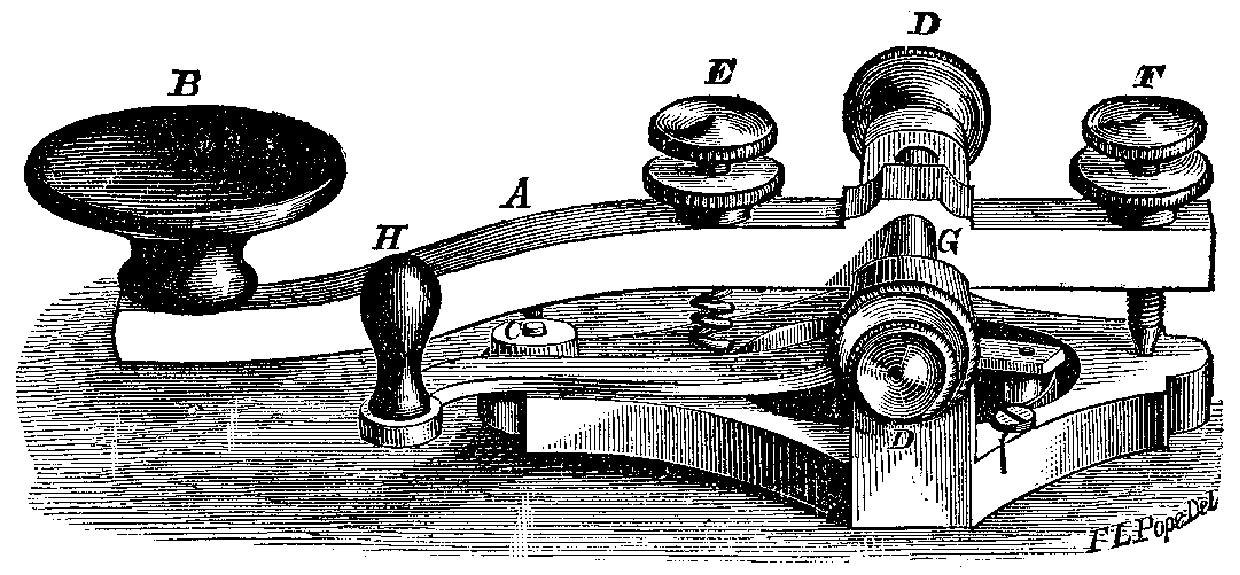
\includegraphics[width=1\textwidth]{animations_figures/morse.pdf}}
\end{figure}

\end{frame}

\begin{frame}
\frametitle{Two strategies for monitoring convergence}

\onslide<2->\textbf{Strategy 2:} monitor the approach to a stationary distribution.

\begin{itemize}
\item<3-> We know asymptotically this will happen.
\item<4-> By design of Metropolis stepping and accept/reject rules, we know the stationary distribution is the posterior.
\end{itemize}

\onslide<1->
\begin{figure}[ht]
\centerline{\includegraphics[width=1\textwidth]{animations_figures/thylacine.jpg}}
\end{figure}

\end{frame}

\begin{frame}
\frametitle{Monitoring convergence of a single chain}

Initial idea:
\begin{itemize}
\item<2-> Compare summaries (mean, variance, etc.) of sampling distribution for a chain at time $t$ with itself at time $t+T$.
\item<3-> If their rate of change is below a threshold $\implies$ convergence.
\end{itemize}

\end{frame}

\begin{frame}
\frametitle{Monitoring convergence of a single chain}
\Large \textbf{Question:} What is the problem with this idea?
\end{frame}

\begin{frame}
\frametitle{Convergence monitoring: Bob's bees}
\onslide<2-> Thought experiment: 
\begin{itemize}
\item<2-> Imagine a house of unknown shape. 
\item<3-> We have an unlimited supply of bees, each equipped with a GPS tracker allowing us to accurately monitor their position.
\item<4-> \textbf{Question:} How can we use these to estimate the shape of the house?
\end{itemize}

\onslide<1->{
\begin{figure}[ht]
\centerline{\includegraphics[width=0.3\textwidth]{animations_figures/lec4_beeAntenna.pdf}}
\end{figure}}

\end{frame}

\begin{frame}
\frametitle{Convergence monitoring: Bob's bees}
\textbf{Answer}: 
\begin{itemize}
\item<2-> Release one (at a random location in the house) and monitor its path over time. 
\item<3-> Stop/collect bee after summary measures of its path stop changing.
\end{itemize}

\end{frame}

\begin{frame}
\frametitle{Convergence monitoring: single bee}

\begin{figure}[t]
\centerline{\animategraphics[width=1\textwidth,controls,buttonsize=1em,buttonfg=0.5]{8}{animations_figures/lec4_beeSingleChaina}{1}{101}}
\end{figure}

\end{frame}

\begin{frame}
\frametitle{Convergence monitoring: single bee, a bit later}

\begin{figure}[t]
\centerline{\animategraphics[width=1\textwidth,controls,buttonsize=1em,buttonfg=0.5]{8}{animations_figures/lec4_beeSingleChainb}{1}{101}}
\end{figure}

\end{frame}

\begin{frame}
\frametitle{Convergence monitoring: single bee, a bit bit later}

\begin{figure}[t]
\centerline{\animategraphics[width=1\textwidth,controls,buttonsize=1em,buttonfg=0.5]{8}{animations_figures/lec4_beeSingleChainc}{1}{111}}
\end{figure}

\end{frame}

\begin{frame}
\frametitle{Convergence monitoring: single bee}
\Large \textbf{Question:} what's the actual shape of the house?

\end{frame}


\begin{frame}
\frametitle{Convergence monitoring: single bee}

\begin{figure}[t]
\centerline{\animategraphics[width=0.8\textwidth,controls,buttonsize=1em,buttonfg=0.5]{8}{animations_figures/lec4_beeSingleChainBuilding}{1}{111}}
\end{figure}

\end{frame}

\begin{frame}
\frametitle{Single chain problems: summary}

\begin{itemize}
\item<2-> One way to monitor convergence is to look for convergence in a single chain's summary statistics.
\item<3-> This method is very susceptible to the curse of hindsight problem (``Now we've definitely converged on the posterior. We hadn't a minute ago.'')
\item<4-> Particularly because chains often get stuck in subregions of $\theta$ space. 
\end{itemize}

\end{frame}

\begin{frame}
\frametitle{The solutions: lots of bees}

\begin{itemize}
\item<2-> Release lots of bees starting at dispersed locations in parameter space.
\item<3-> Stop recording when an individual bee's path is indistinguishable from all others'.
\end{itemize}

\onslide<1->
\begin{figure}[ht]
\centerline{\includegraphics[width=0.3\textwidth]{animations_figures/lec4_bees.pdf}}
\end{figure}

\end{frame}

\begin{frame}
\frametitle{Convergence monitoring: multiple bees}

\begin{figure}[t]
\centerline{\animategraphics[width=0.8\textwidth,controls,buttonsize=1em,buttonfg=0.5]{8}{animations_figures/Lec4_beeMultipleChainWithouta}{1}{81}}
\end{figure}

\end{frame}

\begin{frame}
\frametitle{Convergence monitoring: multiple bees (a lot later)}

\begin{figure}[t]
\centerline{\animategraphics[width=0.8\textwidth,controls,buttonsize=1em,buttonfg=0.5]{8}{animations_figures/lec4_beeMultipleChainWithoutFina}{1}{41}}
\end{figure}

\end{frame}

\begin{frame}
\frametitle{Multiple chain convergence monitoring: summary}

\begin{itemize}
\item<2-> Start a number of chains in random dispersed locations in $\theta$ space. 
\item<3-> Chains do \textit{not} interact with one another (in Metropolis).
\item<4-> Run each sampler until it is hard to distinguish one chain's path from all others'.
\item<5-> Less susceptible to ``curse of hindsight'', since we can see if chains aren't mixing.
\item<6-> Not foolproof! There still may be an area of high probability mass that we miss. However, less likely to fail compared to a single chain.
\item<7-> The more chains, the better!
\end{itemize}

\end{frame}

\begin{frame}
	\frametitle{Judging convergence}
	Single bee in a house.
	
	\begin{figure}[t]
		\centerline{\animategraphics[width=1\textwidth,controls,buttonsize=1em,buttonfg=0.5]{6}{animations_figures/lec5_beeSingleChain}{1}{80}}
	\end{figure}
	
	
\end{frame}

\begin{frame}
	\frametitle{Judging convergence}
	Multiple bees in a house released in a single room.
	
	\begin{figure}[t]
		\centerline{\animategraphics[width=1\textwidth,controls,buttonsize=1em,buttonfg=0.5]{6}{animations_figures/lec5_beeMultipleChainWithout}{1}{40}}
	\end{figure}
	
	
\end{frame}

\begin{frame}
	\frametitle{Judging convergence}
	\textbf{Question:} have we converged?
	
	\onslide<2->
	
	\begin{figure}[t]
		\centerline{\animategraphics[width=1\textwidth,controls,buttonsize=1em,buttonfg=0.5]{6}{animations_figures/lec5_beeMultipleChainWith}{1}{40}}
	\end{figure}
	
\end{frame}

\begin{frame}
	\frametitle{Judging convergence}
	Multiple bees in new house released in highly dispersed rooms.
	
	\begin{figure}[t]
		\centerline{\animategraphics[width=1\textwidth,controls,buttonsize=1em,buttonfg=0.5]{6}{animations_figures/lec5_beeMultipleChainWithoutDispersed}{1}{40}}
	\end{figure}
	
\end{frame}

\begin{frame}
	\frametitle{Judging convergence}
	Multiple bees in new house released in highly dispersed rooms...much later.
	
	\begin{figure}[t]
		\centerline{\animategraphics[width=1\textwidth,controls,buttonsize=1em,buttonfg=0.5]{6}{animations_figures/lec5_beeMultipleChainWithoutDispersedLater}{1}{21}}
	\end{figure}
	
	
\end{frame}


\begin{frame}
\frametitle{Multiple chain convergence monitoring: open questions}

\begin{enumerate}
\item<2-> How to determine ``random dispersed locations'' at which to start the chains?
\begin{itemize}
\item[-]<3-> Ideally use an initial proposal distribution similar to posterior shape.
\item[-]<4-> Otherwise a good rule of thumb is ``Any point you don’t mind having in
a sample is a good starting point'', Charles Geyer.
\end{itemize}
\item<5-> Which summary statistics to monitor to determine convergence?
\item<6-> At what threshold are ``between chain'' statistics sufficiently similar?
\end{enumerate}

\end{frame}

\begin{frame}
\frametitle{Gelman and Rubin's $\hat{R}$}

\begin{itemize}
\item<2-> Gelman and Rubin (1992) had the idea of comparing within-chain to between-chain variability.
\item<3-> They quantified this comparison using:
\begin{equation}
\hat{R} = \sqrt{\frac{W + \frac{1}{n} (B - W)}{W}}
\end{equation}
\item<4-> Where ``within-chain'' variability, $W = \frac{1}{m} \sum\limits_{j=1}^{m} s_j^2$, for $m$ chains.
\item<5-> And ``between-chain'' variability, $B = \frac{n}{m-1} \sum\limits_{j=1}^{m} (\overline{\theta}_j - \overline{\theta})^2$.
\item<6-> When we start $B >> W$ since we start in an overdispersed position.
\item<7-> In convergence $B\rightarrow W \implies \hat{R}\rightarrow 1$ (in practice $\hat{R}<1.1$ usually suffices).
\end{itemize}

\end{frame}


\begin{frame}
\frametitle{Warm up period}
\begin{itemize}
\item<2-> The initial proposal distribution is \textit{not} the posterior.
\item<3-> We therefore discard the beginning part of the chain called the ``warm up'' to lessen the effect of the starting position. 
\item<4-> Typically discard first half of converged chains (can also cut chains in two to monitor intra-chain convergence).
\end{itemize}

\begin{figure}[ht]
\centerline{\includegraphics[width=1.0\textwidth]{animations_figures/warmup.jpg}}
\end{figure}

\end{frame}

\begin{frame}
\frametitle{Warm up period}

\visible<1->{
\begin{figure}[ht]
\centerline{\includegraphics[width=1\textwidth]{animations_figures/lec4_warmUp1.pdf}}
\end{figure}}

\end{frame}

\begin{frame}
\frametitle{Warm up period}

\visible<1->{
\begin{figure}[ht]
\centerline{\includegraphics[width=1\textwidth]{animations_figures/lec4_warmUp2.pdf}}
\end{figure}}

\end{frame}

\section{Adaptive covariance MCMC}
\frame{\tableofcontents[currentsection]}

\begin{frame}
	\frametitle{Inefficient exploration of the typical set by Random Walk Metropolis}
	
	\begin{figure}[t]
		\centerline{\animategraphics[width=0.7\textwidth,controls,buttonsize=1em,buttonfg=0.5]{2}{animations_figures/lec5_MetropolisInefficient}{1}{50}}
	\end{figure}
	
\end{frame}

\begin{frame}
	\frametitle{Adaptive covariance MCMC: adjusting the proposal kernel to posterior geometry}
	
	\begin{itemize}
		\item The problem with RWM is that the proposals - being in random directions - are unlikely by chance to align with areas of high density.
		\item Adaptive covariance MCMC adjusts the proposal kernel dynamically to obtain a higher acceptance probability.
	\end{itemize}
	
\end{frame}

\begin{frame}
	\frametitle{Sketch of adaptive covariance algorithm(s)}
	
	Begin by generating $n$ samples using Random Walk Metropolis. Start with $\Sigma_0 = \text{identity matrix}$. Then,
	
	\begin{enumerate}
		\item Estimate sample mean: $\mu_t = \frac{1}{n}\sum_{i=1}^{t} \theta_i$.
		\item Estimate sample covariance matrix: $\Omega_t =  (\theta^{\{t\}}-\mu_t) (\theta^{\{t\}}-\mu_t)'$.
		\item Proposal kernel: $\Sigma_t = (1-a^t) \Sigma_{t-1} + a^t \Omega_t$.
	\end{enumerate}
	
	$\lim\limits_{t\rightarrow\infty} a^t = 0$ is key to ensuring convergence to posterior distribution.
	
\end{frame}

\begin{frame}
	\frametitle{Adaptive covariance MCMC: adjusting the proposal kernel to posterior geometry}
	
	\begin{figure}[t]
		\centerline{\animategraphics[width=0.7\textwidth,controls,buttonsize=1em,buttonfg=0.5]{2}{animations_figures/adaptive_cartoon}{1}{6}}
	\end{figure}
	
\end{frame}

\begin{frame}
	\frametitle{Adaptive covariance MCMC: summary}
	
	\begin{itemize}
		\item RWM is inefficient due to random directionality of proposals.
		\item Adaptive covariance MCMC dynamically changes proposal kernel to match (global) posterior geometry leading to significant speed ups.
		\item ACMCMC can be used whenever RWM can be $\implies$ very general algorithm; particularly useful for ODE and PDE models, where gradients of solution (necessary for HMC) are expensive.
		\item ACMCMC and loads of other algorithms are available in PINTS: \url{https://github.com/pints-team/pints}.
		\item Problem: adapting to global geometry often leads to very poor local exploration.
	\end{itemize}
	
\end{frame}

\section{Introduction to Hamiltonian Monte Carlo}
\frame{\tableofcontents[currentsection]}

\begin{frame}
	\frametitle{Introduction to Hamiltonian Monte Carlo}
	\begin{itemize}
		\item<2-> Assume a space related to posterior space can be thought of as a landscape.
		\item<3-> Imagine an ice puck moving over the frictionless surface of this terrain.
		\item<4-> At defined time points we measure the location of the puck and instantaneously give the puck a shove in a random direction.
		\item<5-> The locations traced out by the puck represent proposed steps from our sampler.
		\item<6-> Based on the height of the posterior and momentum of the puck we accept/reject steps.
	\end{itemize}
	
\end{frame}

\begin{frame}
	\frametitle{Why does this physical analogy help us?}
	
	\begin{figure}[ht]
		\centerline{\includegraphics[width=0.7\textwidth]{animations_figures/lec5_icePuck.pdf}}
	\end{figure}
	
\end{frame}

\begin{frame}
	\frametitle{Why does this physical analogy help us?}
	
	\begin{itemize}
		\item<2-> Allow the potential energy of the puck to be determined partly by the posterior density.
		\item<3-> $\implies$ puck will move in the ``natural'' directions dictated by the posterior geometry.
		\item<4-> And will visit areas of low NLP $\implies$ high posterior density.
		\item<5-> \textbf{NLP} stands for the \textbf{negative log (un-normalised) posterior},
		
		\begin{equation}
		NLP = - \text{log}\; \left[p(X|\theta) \times p(\theta) \right]
		\end{equation}
		
	\end{itemize}
	
\end{frame}

\begin{frame}
	\frametitle{Simulating the puck's motion in NLP space: start with a posterior}
	
	\begin{figure}[ht]
		\centerline{\includegraphics[width=1\textwidth]{animations_figures/lec5_nlpPosteriorOnly.png}}
	\end{figure}
	
\end{frame}

\begin{frame}
	\frametitle{Simulating the puck's motion in NLP space: find NLP space}
	
	\begin{figure}[ht]
		\centerline{\includegraphics[width=1\textwidth]{animations_figures/lec5_nlpPosterior1.pdf}}
	\end{figure}
	
\end{frame}

\begin{frame}
	\frametitle{Simulating the puck's motion in NLP space: consider a point in posterior space}
	
	\begin{figure}[ht]
		\centerline{\includegraphics[width=1\textwidth]{animations_figures/lec5_nlpPosterior2.pdf}}
	\end{figure}
	
\end{frame}

\begin{frame}
	\frametitle{The path traced out for 100 different shoves from same distribution}
	
	\begin{figure}[t]
		\centerline{\animategraphics[width=1\textwidth,controls,buttonsize=1em,buttonfg=0.5]{2}{animations_figures/lec5_puckPath}{1}{26}}
	\end{figure}
	
\end{frame}

\begin{frame}
	\frametitle{The HMC algorithm}
	\onslide<2-> The HMC algorithm works as follows,
	
	\begin{itemize}
		\item<3-> Start at random location $\theta_0$.
		\item<4-> For $i=1,...,N$ do:
		\begin{enumerate}
			\item<5-> Give puck random initial momentum, $k\sim N(0,\Sigma)$.
			\item<6-> Simulate puck's movement across NLP surface for a fixed time $T$ (number of discrete steps of numerical integration algo).
			\item<7-> Compute a ratio:
			
			\begin{equation}
			r = \frac{p(\theta_t|X)}{p(\theta_{t-1}|X)} \times \frac{p(k')}{p(k)}
			\end{equation}
			
			where $k$ is the final momentum.
			
			\item<8-> If $r > u \implies$ move to $\theta_{t}$, otherwise return to $\theta_{t-1}$.
		\end{enumerate}
	\end{itemize}
	
\end{frame}

\begin{frame}
	\frametitle{The HMC algorithm}
	
	\begin{figure}[t]
		\centerline{\animategraphics[width=1\textwidth,controls,buttonsize=1em,buttonfg=0.5]{12}{animations_figures/lec6_hmc_a}{1}{154}}
	\end{figure}
	
\end{frame}

\begin{frame}
	\frametitle{The HMC algorithm}
	
	\begin{figure}[t]
		\centerline{\animategraphics[width=1\textwidth,controls,buttonsize=1em,buttonfg=0.5]{12}{animations_figures/lec6_hmc_b}{1}{154}}
	\end{figure}
	
\end{frame}

\begin{frame}
	\frametitle{The HMC algorithm}
	
	\begin{figure}[t]
		\centerline{\animategraphics[width=1\textwidth,controls,buttonsize=1em,buttonfg=0.5]{12}{animations_figures/lec6_hmc_c}{1}{2}}
	\end{figure}
	
\end{frame}


\begin{frame}
	\frametitle{Simulating the puck's motion in NLP space: randomly shoving the puck at intervals of 50 steps}
	
	\begin{figure}[t]
		\centerline{\animategraphics[width=1\textwidth,controls,buttonsize=1em,buttonfg=0.5]{5}{animations_figures/lec6_HMC}{1}{109}}
	\end{figure}
	
\end{frame}

\begin{frame}
	\frametitle{RWM and Gibbs performance}
	
	\begin{figure}[t]
		\centerline{\animategraphics[width=1\textwidth,controls,buttonsize=1em,buttonfg=0.5]{2}{animations_figures/lec5_gibbsBirdsBothCorrelateda}{1}{30}}
	\end{figure}
	
\end{frame}

\begin{frame}
	\frametitle{Hamiltonian Monte Carlo performance}
	
	\begin{figure}[t]
		\centerline{\animategraphics[width=0.6\textwidth,controls,buttonsize=1em,buttonfg=0.5]{2}{animations_figures/lec5_birdsHMC}{1}{30}}
	\end{figure}
	
\end{frame}

\begin{frame}
	\frametitle{Hamiltonian Monte Carlo: summary}
	
	\begin{itemize}
		\item<2-> Imagine a puck sliding across a frictionless surface of the negative log posterior (NLP).
		\item<3-> Give puck random shoves at predefined time intervals, and simulate path of puck for predefined time interval.
		\item<4-> Puck will tend to visit areas of low NLP which correspond to areas of high posterior density!
		\item<5-> Algorithm often performs considerably better than Random Walk Metropolis or Gibbs.
		\item<6-> Stan uses a fancy variant of HMC known as NUTS (No U-Turn Sampler) that determines the optimal time intervals to simulate puck for.
	\end{itemize}
	
\end{frame}


\section{Ordinary differential equations}
\frame{\tableofcontents[currentsection]}

\begin{frame}
	\frametitle{Example: bacterial growth}
	\begin{itemize}
		\item<2-> We carry out experiments where we inoculate agar plates with bacteria at time 0.
		\item<3-> At pre-defined time intervals we count the number of bacteria on each plate, $N(t)$.
		\item<4-> Suppose we want to model bacterial population growth over time.
	\end{itemize}
	
	\onslide<1->
	\begin{figure}[ht]
		\centerline{\includegraphics[width=1\textwidth]{animations_figures/bacteria.png}}
	\end{figure}
	
\end{frame}

\begin{frame}
	\frametitle{Example: bacteria growth data}
	
	\begin{figure}[ht]
		\centerline{\includegraphics[width=1\textwidth]{animations_figures/lec7_odeSingle.pdf}}
	\end{figure}
	
\end{frame}

\begin{frame}
	\frametitle{Example: bacterial growth model}
	\begin{itemize}
		\item<2-> Assume the following model for bacterial population growth:
	\end{itemize}
	
	\onslide<3->
	\begin{equation}
	\frac{\mathrm{d}N}{\mathrm{d}t} = \alpha N (1-\beta N)
	\end{equation}
	
	\onslide<4->
	where $\alpha>0$ is the rate of growth due to bacterial cell division, and $\beta>0$ measures the reduction in growth rate due to ``crowding''. 
	
	\onslide<5->
	\textbf{Question:} how should we infer the parameters of this model?
	
\end{frame}

\begin{frame}
	\frametitle{Example: bacterial growth model}
	\onslide<2->
	\textbf{Answer:} assume measurement error around true value:
	
	\onslide<3->
	\begin{equation}
	N^*(t) \sim \text{normal}(N(t), \sigma)
	\end{equation}
	
	\onslide<4->
	where
	\begin{itemize}
		\item<5-> $N^*(t)$ is the \textbf{measured} count of bacteria at time $t$.
		\item<6-> $N(t)$ is the solution to the ODE at time $t$ (true number of bacteria on plate).
		\item<7-> $\sigma>0$ measures the magnitude of the measurement error about the true value.
	\end{itemize}
	
	\onslide<8-> \textbf{Question:} how does this model work?
	
\end{frame}

\begin{frame}
	\frametitle{Example: bacterial growth model}
	Start with true number of bacterial cells, $N(t)$.
	
	\onslide<2->
	\begin{figure}[ht]
		\centerline{\includegraphics[width=1\textwidth]{animations_figures/lec7_odeSingleBulding1.pdf}}
	\end{figure}
	
\end{frame}

\begin{frame}
	\frametitle{Example: bacterial growth model}
	Overlay sampling distribution representing measurement error.
	
	\begin{figure}[ht]
		\centerline{\includegraphics[width=1\textwidth]{animations_figures/lec7_odeSingleBulding2.pdf}}
	\end{figure}
	
\end{frame}

\begin{frame}
	\frametitle{Example: bacterial growth model}
	And data generated from this process.
	
	\begin{figure}[ht]
		\centerline{\includegraphics[width=1\textwidth]{animations_figures/lec7_odeSingleBulding3.pdf}}
	\end{figure}
	
\end{frame}

\begin{frame}
	\frametitle{Example: bacteria growth model inference}
	\onslide<2-> Remember we are using a normal likelihood:
	
	\onslide<3->
	\begin{equation}
	N^*(t) \sim \text{normal}(N(t), \sigma)
	\end{equation}
	
	\onslide<4->
	$\implies$ likelihood for all observations:
	
	\onslide<5->
	\begin{equation}
	L(N(t),\sigma) = \prod_{t={t_1}}^{T} \frac{1}{\sqrt{2\pi\sigma^2}} exp\left[\frac{-(N^*(t) - N(t))^2}{2\sigma^2}\right]
	\end{equation}
	
	\onslide<6->
	\textbf{Question:} how do we calculate $N(t)$?
	
\end{frame}

\begin{frame}
	\frametitle{Example: bacteria growth model inference}
	
	\begin{equation}
	\frac{\mathrm{d}N}{\mathrm{d}t} = \alpha N (1-\beta N)
	\end{equation}
	
	\begin{itemize}
		\item<2-> In most ODE models, the mean $N(t)$ cannot be solved for exactly so we \textbf{can't write down a ``closed-form'' expression for the likelihood.}
		\item<3-> $\implies$ approximate answer using a numerical method.
		\item<4-> However any solution for $N(t)$ - exact or numerical - depends on the parameters of the ODE model. For our example:
		
		\onslide<5->
		
		\begin{equation}
		N(t) = f(t,\alpha,\beta)
		\end{equation}
		
	\end{itemize}
	
	\vspace{0.2cm}
	
	\onslide<6->
	\textbf{Question:} how do we do MCMC in this setting?
	
\end{frame}

\begin{frame}
	\frametitle{Example: bacteria growth model inference}
	
	\onslide<2-> For example, in Random Walk Metropolis:
	
	\begin{itemize}
		\item<3-> Start at random location in $(\alpha,\beta,\sigma)$ space.
		\item<4-> For t=1,...,T do:
		\begin{enumerate}
			\item<5-> Propose a new location $(\alpha',\beta',\sigma')$ using a jumping distribution.
			\item<6-> Numerically (or analytically) integrate ODE to solve for $N(t,\alpha',\beta')$.
			\item<7-> Calculate un-normalised posterior at proposed location $\implies$ calculate $r$.
			\item<8-> Based on $r$ move to new location or stay at original.
		\end{enumerate}
	\end{itemize}
	
	\onslide<9->
	$\implies$ at every step we must solve ODE for $N(t)$; can be computationally expensive!
	
\end{frame}

\begin{frame}
	\frametitle{Issues with inference for ODEs and PDEs}
	\begin{itemize}
		\item<2-> ODE models are very often non-identifiable $\implies$ need to reparameterise model.
		\item<3-> (Linked) ODE models can be slower to converge than simpler models $\implies$ need to run MCMC for longer before $\hat{R}<1.1$ achieved.
	\end{itemize}
	
	\onslide<4->
	$\implies$ important that we ``know'' our model well before we start to do inference explicitly.
	
	\onslide<5-> Worth putting energy into mathematical analysis before trying MCMC. 
	
\end{frame}


\begin{frame}
	\frametitle{Inference for ODEs: summary}
	\begin{itemize}
		\item<2-> ODE models are no harder to formulate than ``traditional'' problems.
		\item<3-> However for ODE models we cannot typically write down a ``closed-form'' expression for the likelihood.
		\item<4-> $\implies$ use integrator to numerically solve for mean for each set of parameters.
		\item<5-> Posteriors for ODE models are often of a more complex geometry than regular models and are often unidentified.
		\item<6-> Check out: \url{https://github.com/pints-team/pints} for ODE inference.
	\end{itemize}
	
\end{frame}


\section{Approximate Bayesian computation}
\frame{\tableofcontents[currentsection]}

\begin{frame}
	\frametitle{Intractable likelihood}
	A class of models have the property that the likelihood is too costly to evaluate exactly,
	
	\begin{itemize}
		\item<2-> Population genetics,
		\item<3-> Evolutionary biology,
		\item<4-> Epidemiology,
		\item<5-> Spatial models (e.g. cellular automata, cellular Potts, CHASTE),
		\item<6-> Models involving stochasticity.
	\end{itemize}
	
	\onslide<7-> However it may be (relatively) inexpensive to run a model for a given parameter set $\theta$.
	
\end{frame}

\begin{frame}
	\frametitle{Example: stochastic Lotka-Volterra}
	Predator $Y$ and prey $X$,
	
	\begin{align}
	X &\xrightarrow{c_1} 2 X\\ 
	X + Y &\xrightarrow{c_2} 2Y\\
	Y &\xrightarrow{c_3} \emptyset
	\end{align}
	
	$\implies$ can simulate dynamics exactly using the Gillespie algorithm, but difficult to determine $p(\boldsymbol{X},\boldsymbol{Y}|c_1,c_2,c_3)$.
	
\end{frame}

\begin{frame}
	\frametitle{Basic ABC algorithm}
	\textbf{Question:} how can we infer $(c_1,c_2,c_3)$?
	
	\vspace{0.2cm}
	
	\onslide<2-> \textbf{Idea}: iterate the following, 
	\begin{enumerate}
		\item<3-> Simulate from algorithm using $(c_1,c_2,c_3)\sim \pi(.)$, the prior.
		\item<4-> If $||T\boldsymbol{(X,Y)}_{sim} - T\boldsymbol{(X,Y)}||<\epsilon \implies$ accept parameters.
		\item<5-> Else reject.
	\end{enumerate}
	
	\onslide<6->
	Where $T(.)$ is some type of informative summary statistic. For example, here we might choose the sum of squared errors.
	
\end{frame}

\begin{frame}
	\frametitle{Basic ABC algorithm: the role of $\epsilon$}
	\textbf{Test:} simulate data from stochastic Lotka-Volterra model where, $(c_1,c_2,c_3) = (10,0.01,10)$, and $(X_0,Y_0) = (1000,1000)$ for $T=0.1$.
	
	\onslide<2->
	\begin{figure}[ht]
		\centerline{\includegraphics[width=0.9\textwidth]{animations_figures/predatorPrey.pdf}}
	\end{figure}
	
	\onslide<3->
	\textbf{Question:} how does choice of $\epsilon$ affect posterior?
	
\end{frame}

\begin{frame}
	\frametitle{Basic ABC: high $\epsilon$}
	
	\onslide<2->
	\begin{figure}[ht]
		\centerline{\includegraphics[width=1\textwidth]{animations_figures/predatorPreyHighEpsilon.pdf}}
	\end{figure}
	
	\onslide<3-> quick to run but $\implies$ approximate posterior same as priors!
\end{frame}

\begin{frame}
	\frametitle{Basic ABC: low $\epsilon$}
	
	\onslide<1->
	\begin{figure}[ht]
		\centerline{\includegraphics[width=1\textwidth]{animations_figures/predatorPreyLowEpsilon.pdf}}
	\end{figure}
	
	\onslide<2-> slow to run but $\implies$ approximate posterior near true posterior!
\end{frame}

\begin{frame}
	\frametitle{ABC: summary}
	
	\begin{itemize}
		\item<2-> ABC can be used to estimate approximate posteriors for some models where likelihood is intractable to calculate,
		\item<3-> so long as the time for a simulation is $\mathcal{O}(\text{seconds})$.
		\item<4-> Many variants of ABC exist, for example, Sequential/Particle MC, MCMC, regression $\implies$ generally help with rate of convergence to the posterior.
		\item<5-> Often useful (and less time intensive) step towards full Bayesian analysis of ODE and PDE models, and can help with questions around model identification.
		\item<6-> For slower simulations, either require large parallelism (e.g. ARCUS) or use more approximate methods (e.g. surrogate models).
	\end{itemize}
	
\end{frame}

\begin{frame}
\frametitle{Summary}

\begin{enumerate}
\item<2-> Sampling can be used to gain insight into a distribution.
\item<3-> Independent sampling from posterior not generally possible $\implies$ shift to dependent sampling.
\item<4-> Random Walk Metropolis is a MCMC algorithm that allows \textit{dependent} sampling from the posterior.
\item<5-> The efficiency of Metropolis depends on choosing the right step size.
\item<6-> Monitoring of sampler's convergence to the posterior is non-trivial.
\item<7-> The use of multiple chains makes it harder to make a mistake although not impossible.
\item<8-> Adaptive covariance MCMC and HMC can speed up sampling dramatically.
\end{enumerate}

\end{frame}


\begin{frame}
	\frametitle{Not sure I understand?}
	Hamiltonian Monte Carlo.
	
	\begin{figure}[ht]
		\centerline{\includegraphics[width=0.3\textwidth]{animations_figures/lec5_icePuck.pdf}}
	\end{figure}
	
	Hamilton in Monte Carlo.
	
	\begin{figure}[ht]
		\centerline{\includegraphics[width=0.3\textwidth]{animations_figures/hamiltonMonteCarlo1.jpg}}
	\end{figure}
	
	
\end{frame}

\end{document}
